\chapter{Writing a thesis in LaTeX}
A LaTeX document class has been developed, which follows the guidelines
described in \cite{kulemtgl}. The usage of this class is described in
\Cref{cha:kulemt}. \Aref{app:template} contains a typical LaTeX template. The
result can be customised and adapted to the master's programme guidelines with
the class options. Additional functionality is available through numerous LaTeX
packages (cf.\ \Sref{sec:packages}). Just make sure that the final result still
conforms to the guidelines.

The following sections assume you already have a working LaTeX installation. If
this is not the case on a Linux based distribution, first check the
distribution documentation. Otherwise consult the TeX-FAQ\,\cite{texfaq} for
installing a LaTeX distribution for your system.

If you are not (yet) familiar with LaTeX, you should first have a look at the
documentation of the TeX Users Group \cite{tugstart}. It also contains a list
of on-line tutorials and manuals. The most popular tutorial is probably
\citewithtitle{lshort}. The next section contains some extra information on how
to install LaTeX packages. It also lists some typically useful packages.

\section{Using LaTeX packages}\label{sec:packages}
The document class \cls{kulemt} uses some standard LaTeX packages (such as
\pkg{babel} and \pkg{graphicx}) and is based on the document class
\cls{memoir}, so it also includes all packages included or emulated by
\cls{memoir}\,\footnote{The \cls{memoir} class includes or emulates since
  2018-12-12 at least the packages \pkg{abstract}, \pkg{appendix}, \pkg{array},
  \pkg{booktabs}, \pkg{ccaption}, \pkg{changepage}, \pkg{chngcntr},
  \pkg{chngpage}, \pkg{crop}, \pkg{dcolumn}, \pkg{delarray}, \pkg{enumerate},
  \pkg{epigraph}, \pkg{ifmtarg}, \pkg{index}, \pkg{makeidx}, \pkg{moreverb},
  \pkg{mparhack}, \pkg{needspace}, \pkg{newfile}, \pkg{nextpage},
  \pkg{pagenote}, \pkg{parskip}, \pkg{patchcmd}, \pkg{setspace},
  \pkg{shortvrb}, \pkg{showidx}, \pkg{tabularx}, \pkg{titleref}, \pkg{titling},
  \pkg{tocbibind}, \pkg{tocloft}, \pkg{tocvsec2}, \pkg{verbatim}, and
  \pkg{verse}.}. The exact list of packages included or emulated in
\cls{memoir} can always be found in the log file after a LaTeX run. The
emulation not always corresponds to the latest version of the package, but the
main functionality is usually present. So before installing a new package,
first check the \cls{memoir} manual\,\cite{memman} to see if the functionality
is not already present in the document class.

\subsection{Installing a LaTeX package}\label{sec:install}
Most of the packages listed below are included in a standard LaTeX
installation, with the exception of the \pkg{kulemt} package. But in case you
need to install a package yourself, you can follow the instructions found in
the TeX-FAQ\,\cite{texfaq} under the heading \enquote{Shortcuts to installing
  files}. If you only can or want to install packages for your personal use,
make sure you also read \enquote{Private installations of files}.

The installation of the document class \cls{kulemt} is done in the same way as
the installation of any other package. The only difference is the fact that its
source is currently not available from \acro{CTAN} or a Linux distribution but
from a local web server\,\citeurl{pkg:kulemt}.

\subsection{Useful extra LaTeX packages}
A lot of packages are available from \acro{CTAN}\,\cite{CTAN}, which can help
you to make your text easier to understand or more impressive. Many of them are
installed by default in a traditional LaTeX installation. Some typical examples
are given in \tref{tab:otherpack}.
\begin{table}
  \caption{Packages which can be useful to extend the \cls{kulemt} class.}
  \label{tab:otherpack}
  \centering
  \renewcommand*\thefootnote{\fnsymbol{footnote}}
  \begin{tabular}{@{}ll@{}}
    \toprule
    Package        & Description \\
    \midrule
    \pkg{hyperref} & Provide hyperlinks in \PDF\ files \\
    \pkg{microtype}& Enhance the typographic quality of your text \\
    \pkg{amsmath}  & Extra mathematical constructs \\
    \pkg{amssymb}  & Extra mathematical symbols\footnotemark[1] \\
    \pkg{rotating} & Rotating material, e.g., figures en tables \\
    \pkg{listings} & Typeset programming code \\
    \pkg{nomencl}  & Produce lists of symbols (nomenclature) \\
    \pkg{tikz}     & Create graphics in LaTeX \\
    \pkg{siunitx}  & Consistent use of SI units \\
    \pkg{biblatex} & Sophisticated bibliographies in LaTeX \\
    \pkg{cite}     & Better references (when using BibTeX) \\
    \bottomrule \addlinespace
    \multicolumn2{l}{\footnotemark[1] \footnotesize
      A list of all kind of symbols is found in \citewithtitle{symbols}.} \\
  \end{tabular}
\end{table}
The loading order can be important for some combination of packages:
packages, which extend or redefine commands of other packages, must be
loaded after those packages.

If you are making a \PDF\ file for on-line distribution, the use of the
\pkg{hyperref} package\,\cite{pkg:hyperref} is a must. It not only
automatically generates the bookmarks, but it also gives you all the linking
facilities required in modern on-line documents.

The \pkg{microtype} package\,\cite{pkg:microtype} enhances the typographic
quality of the text. The most important enhancements provided by the package
are character protrusion and font expansion. Character protrusion lets some
characters slightly enter the margin to provide optical margins. Font expansion
creates fonts which are a little bit narrower or wider. It generates more equal
interword spacing and it provides also more flexibility to avoid hyphenation.
Both effects are illustrated in \fref{fig:microtype}.
\begin{figure}
  \centering
  \setlength{\fboxsep}{9pt}
  \fbox{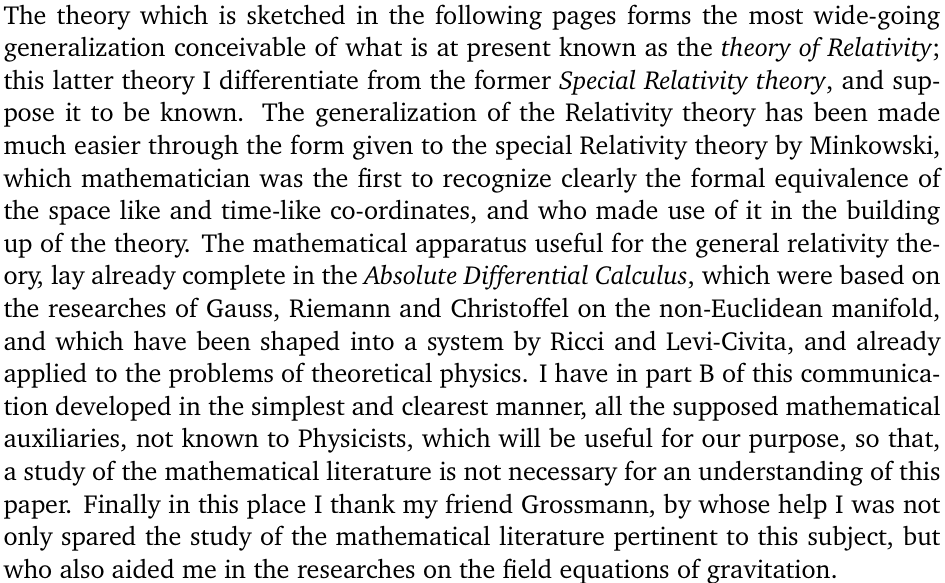
\includegraphics[width=.95\columnwidth]{microtype_off.png}}
  \vspace{0pt}
  \subcaption{Text typeset without using \pkg{microtype}.}
  \par\bigskip
  \fbox{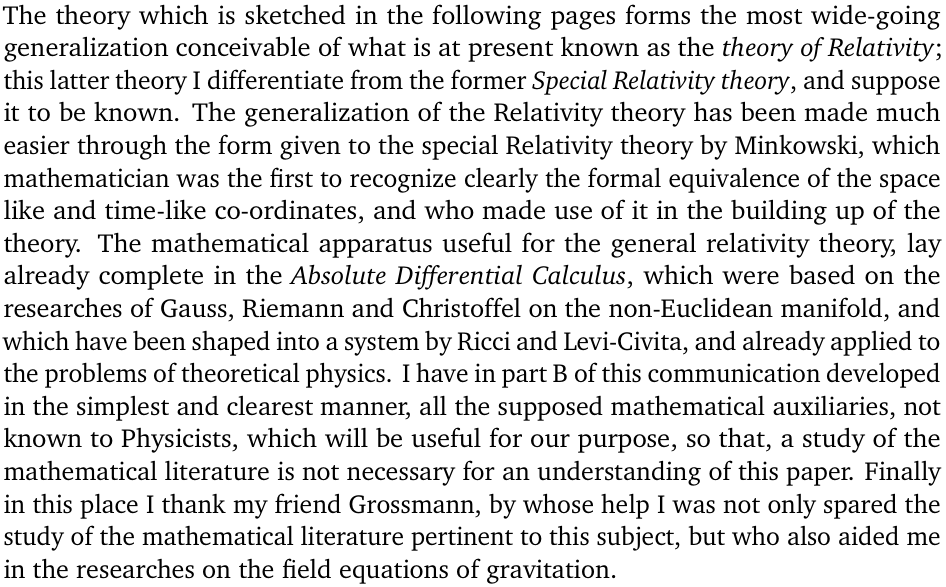
\includegraphics[width=.95\columnwidth]{microtype_on.png}}
  \vspace{0pt}
  \subcaption{The same text typeset using \pkg{microtype} (character
    protrusion \& font expansion).}
  \caption[The effect of using the \pkg{microtype} package.]{The effect of
    using the \pkg{microtype} package. These examples are based on
    \url{https://gist.github.com/AndiH/8b65adbeb77b00c4b970}.}
  \label{fig:microtype}
\end{figure}
It works best with \prog{pdflatex} or \prog{lualatex}.

LaTeX is basically a document processing system for text. The easiest way to
include graphics or diagrams, is to generate them with an external processor
and then include them with `\verb"\includegraphics"'\,\footnote{This command is
  defined by the \pkg{graphicx} package, which is already preloaded by the
  \cls{kulemt} class.}. But external processors mostly use different fonts and
scaling, which clashes with the look of the rest of your document. An
alternative is to use the \pkg{tikz} package\,\cite{pkg:tikz} where drawing is
done using TeX commands, such as in \fref{fig:compile}. Its manual of more than
1300~pages shows how to generate graphics for different domains. Furthermore,
\acro{CTAN} holds more than 150~packages enhancing \pkg{tikz} or making use of
it \cite{CTAN-tikz}.

\section{Selecting fonts}\label{sec:fonts}
The thesis guidelines only give some general hints about fonts, but they don't
enforce specific fonts, except for the title page and the cover page. Not only
a text font must be selected but also a matching math font. Even if you don't
use formulas or equations, a math font is often needed for subscripts or
superscripts.

Two types of font formats can be used: the older Type1 format and the modern
OpenType format (\acro{OTF} or \acro{TTF}). Modern operating system fonts, such
as \texttt{Cambria} on Windows (or the free compatible \texttt{Caladea}) or
\texttt{Geneva} on MacOS, are usually only available in the OpenType format.
Both font formats can be used by \prog{lualatex} and \prog{xelatex} while
\prog{pdflatex} can only use Type1 fonts. A list of available fonts in a
standard LaTeX system can be found in \citewithtitle{fontcatalogue}.

You can select your own combination of fonts using standard LaTeX packages. If
no fonts are defined, the default LaTeX fonts (Latin Modern) are used. Recent
packages are aware of the LaTeX engine you use and automatically switch between
the font formats. Often they also provide suitable math fonts. Some examples
are: \pkg{erewhon} (Utopia based), \pkg{libertinus} (used in this manual),
\pkg{newpx} (Palatino based), \pkg{newtx} (Times based), and \pkg{XCharter}
(Charter based). The wrapper-type package \pkg{fontsetup} may simplify choosing
between OpenType fonts with math counterparts. For more information, have a
look at the documentation of these packages on \acro{CTAN}~\cite{CTAN} or via
\prog{texdoc}~\cite{texdoc}. An almost complete overview of all possibilities
is described in a recent \citewithtitle{companion3}.

\section{Adding a bibliography}\label{sec:bib}
The bibliography can be input as a list in the text, using the
\env{thebibliography} environment. A better way to generate a bibliography is
with the help of the BibTeX programme~\cite{tamethebeast} or the Biber
programme~\cite{pkg:biber}. The latter requires the use of the \pkg{biblatex}
package\,\cite{pkg:biblatex}. The bibliographic data is stored in one or more
bibliographic files (files with extension `\file{.bib}'). Apart from a personal
data file, existing data files can be used for some disciplines.
For more information, please consult the website \citewithtitle[lesson~12
(Citations and references)]{learnlatex}. It will also help you choose between
the BibTeX workflow and \pkg{biblatex}. 

The master's programme guidelines or the thesis supervisor determine which
bibliography style to use. If none is specified, you can choose whichever you
find most suited for your text.

\section{Using \prog{latex}, \prog{pdflatex}, \prog{lualatex} or
  \prog{xelatex}?}\label{sec:engine}
The traditional way to compile a LaTeX file uses the \prog{latex} programme. It
outputs the typeset document to a \file{.dvi} file, which is rather TeX
specific. So usually this is converted to a PostScript file using \prog{dvips}
or a \PDF\ file using \prog{dvips}~+~\prog{dvipdfmx}. However, since every
master's thesis must also be submitted electronically in \PDF~format, there is
no reason to take the PostScript route unless your text depends on packages
which work only with PostScript output, such as \pkg{psfrag} or all kind of
PSTricks packages. But often valid or even better replacements exist, such as
the \pkg{tikz} package\,\cite{pkg:tikz}. Conversion tools may also be available
(e.g., the \pkg{pst-pdf} package).

\begin{figure}
  \newcommand*\pnode[2][]{\path (#2) node[rectangle, draw, thick,
    minimum width=20\unitlength, minimum height=10\unitlength,#1]}
  \newcommand*\fnode[2][]{%
    \draw[thick,#1] (#2) +(-5,5) -- +(5,5) --
      +(5,-5) .. controls +(-2,2)  and +(2,1)  ..
      +(0,-5) .. controls +(-2,-1) and +(2,-2) ..
      +(-5,-5) -- cycle;
    \path (#2) node[rectangle, minimum width=10\unitlength,
                    minimum height=10\unitlength, align=center]}
  \setlength\unitlength{1mm}
  \centering
  \begin{tikzpicture}[x=\unitlength, y=\unitlength, semithick, >=stealth']
    \ttfamily\small
    %% program nodes
    \pnode[align=center]{30,17}(pltx){pdflatex\\lualatex\\xelatex};
    \pnode[dashed,align=center]{80,10}(pbtx){bibtex\\biber};
    %% file nodes
    \fnode{ 5,25}(ftex){.tex};
    \fnode{55,25}(fpdf){.pdf};
    \fnode{55,10}(faux){.aux\\[-1ex]\textrm{\ldots}};
    \fnode[dashed]{102,10}(fbbl){.bbl};
    %% arrows
    \draw[->] (ftex.east) -- ++(5,0) |- ($(pltx.west)+(0,2.5)$);
    \draw[->] ($(pltx.east)+(0,2)$)  -- ++(5,0) |- (fpdf.west);
    \draw[->] ($(pltx.east)+(0,-2)$) -- ++(5,0) |- (faux.west);
    \draw[->] (faux.east) -- ++(4,0) |- (15,2)
              |- ($(pltx.west)+(0,-2.5)$);
    \draw[dashed,->] ($(faux.east)+(4,0)$)  -- (pbtx);
    \draw[dashed,->] (pbtx) -- (fbbl);
    \draw[dashed,->] (fbbl.east) -- ++(5,0) |- (12,0) |- (pltx.west);
  \end{tikzpicture}\medskip
  \caption[Steps to compile a LaTeX file]{Steps to compile a LaTeX file. The
    dashed part is needed only if a bibliography is used. As long as the
    \file{.bbl} file or internal files (\file{.aux}, \file{.toc}, \file{.lof},
    \file{.lot}, \ldots) change, (\file{pdf}/\file{lua}/\file{xe})\file{latex}
    must be invoked again. If you use an intelligent editor, it will tell you
    when an extra iteration is needed.}%
  \label{fig:compile}
\end{figure}
If you want a \PDF~file as a result, it's easier to use \prog{pdflatex}, as
illustrated in \fref{fig:compile}. But \prog{pdflatex} has other advantages
too. It uses the pdfTeX engine, which is an enhanced implementation of the TeX
engine used by \prog{latex}. Therefore more advanced features, such as breaking
hyperlinks (\pkg{hyperref} package) or font expansion (\pkg{microtype}
package), are only possible with the pdfTeX engine. Additionally, the pdfTeX
engine can directly include images in the \acro{JPEG} or \acro{PNG} file format
as well as other \PDF\ files. Simple PostScript (e.g., as generated by
MetaPost) can also be included but general \acro{EPS} (Encapsulated Postscript)
not. You'll have to convert the latter to \PDF\ with the \prog{epstopdf}
programme.

A modern installation also provides the \prog{xelatex} and \prog{lualatex}
programmes, based respectively on the XeTeX and the LuaTeX engine. The XeTeX
engine is derived from the TeX engine and supports almost any system font (cf.\
\Sref{sec:fonts}). The LuaTeX engine is a greatly extended version of pdfTeX
using Lua as an embedded scripting language. Some packages use the Lua
interpreter to perform more complex computations than any other TeX based
engine can do. It also enables \prog{lualatex} to use modern fonts (cf.\
\Sref{sec:fonts}).

When you use a LaTeX-oriented editor or online software, such as Overleaf,
selecting the engines or the programmes to run, can be changed in the settings.

A final word of advice: to avoid errors and text drifting to other places,
don't switch between engines gratuitously.


%%% Local Variables: 
%%% mode: latex
%%% TeX-master: "kulemt"
%%% ispell-local-dictionary: "british"
%%% End: 
